\section{Redegørelse af et ANN netværk}

\subsection{ANN's baggrund}
Et ANN(Artificial Neural Network) er en form for kunstig intellegens, hvor man prøver at efterligne den menneskelige hjerne
ved at lave simple versioner af det netværk af de mange milliarder neuroner der findes i den menneskelige hjerne.
Ligesom hvor en biologisk menneskehjerne har neuroner og synapser med forskellige styrker, så har et ANN også det, dog lidt simplere
så man kan tillægge værdier til de forskellige neuroner og synapser.

\subsection{Strukturen bag et ANN}
I den menneskellige hjerne er der som sagt milliarder af forskellige neuroner \footcite{DDOhjerne}.
I et ANN laver man ikke ligeså mange
neuroner som i en rigtig hjerne, da det er umuligt med den teknologi vi har i dag, men det er stadigvæk i fokus at lave et netværk med så mange neuroner
som muligt.
Derfor er det vigtigt at disse neuroner er matematisk set meget simple, så det er nemt for en moderne computer bare at blæse gennem matematikken
i et ANN. Så den strukter man så har valgt bag én neuron i et givet ANN er figur 1.

\begin{figure}
\label{neuron}
\caption{Model af en neuron}
\LARGE
\begin{center}
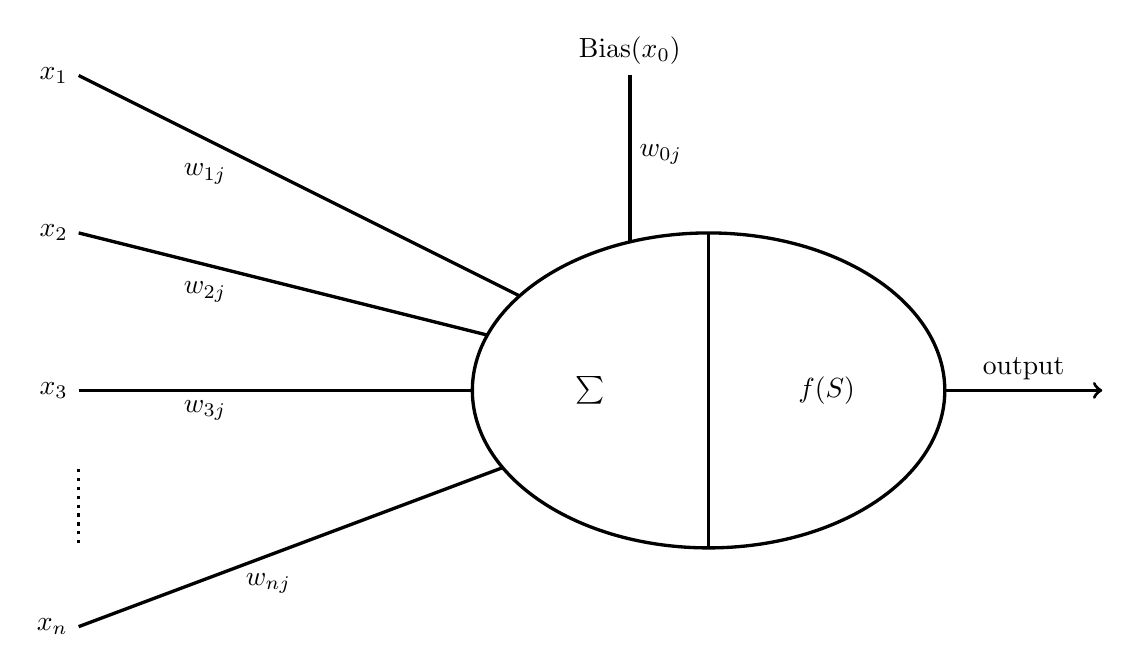
\begin{tikzpicture}

        \draw[very thick] (-1, 4) node[anchor=south]{Bias($x_0$)} -- (-1, 0);
        \draw[very thick] (-8, 4) node[anchor=east]{$x_1$} -- (0, 0);
        \draw[very thick] (-8, 2) node[anchor=east]{$x_2$} -- (0, 0);
        \draw[very thick] (-8, 0) node[anchor=east]{$x_3$} -- (0, 0);
        \draw[very thick, dotted] (-8, -1) -- (-8, -2);
        \draw[very thick] (-8, -3) node[anchor=east]{$x_n$}-- (0, 0);

        \node[anchor=west] at (-1, 3){$w_{0j}$};
        \node[anchor=north east] at (-6, 3){$w_{1j}$};
        \node[anchor=north east] at (-6, 1.5){$w_{2j}$};
        \node[anchor=north east] at (-6, 0){$w_{3j}$};
        \node[anchor=north west] at (-6, -2.2){$w_{nj}$};

        \draw[very thick, fill=white] (0, 0) ellipse (3 and 2);
        \draw[very thick] (0, 2) -- (0, -2);
        
        \node at (-1.5, 0){$\sum$};
        \node at (1.5, 0){$f(S)$};

        \draw[very thick, ->] (3, 0) -- (4, 0) node[anchor=south]{output} -- (5, 0);

\end{tikzpicture}
\end{center}
\normalsize

\end{figure}

Hvor alle $x_n$ er outputs fra andre neuroner der er tilsluttet denne neuron via synapser, $w_{nj}$ er såkaldte vægte der angiver hvor
forstærket signalet er fra outputtet af sidste neuron og bias er en værdi der der enten vil øge eller
sænke outputtet af en given neuron. Det der så sker inde i neuronen er to ting. \\
Først bliver alle inputs ganget sammen med deres vægte og summeret op. \\
Derefter bliver der ført en såkaldt "Activation function" der typisk bare normaliserer
summationen mellem f.eks 0 og 1\footcite{ANN11}. Her betragter jeg bare logistisk vækst med et maksimum på 1 som min activation function.
Funktionen vil så tage et vilkårligt tal og så spytte et andet tal ud der ligger mellem 0 og 1
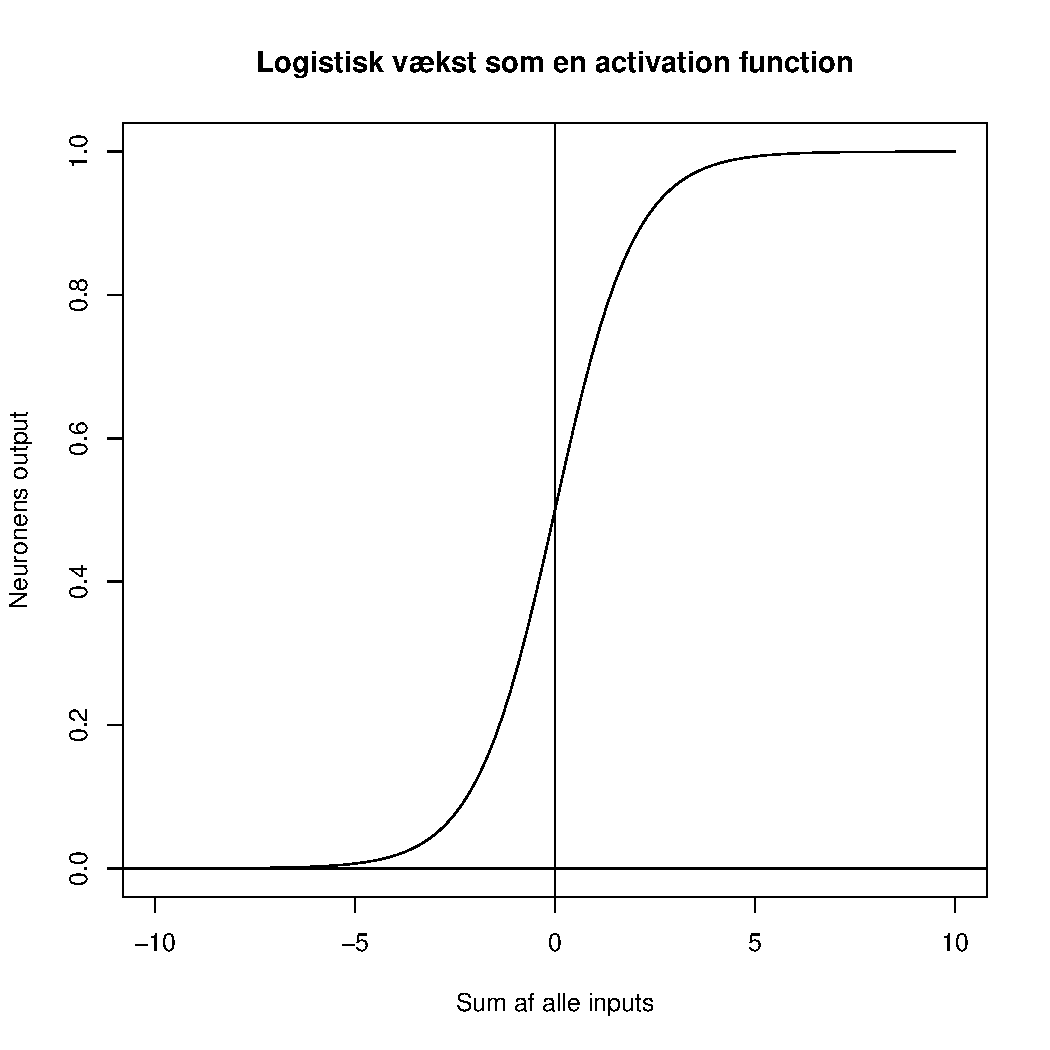
\includegraphics[width=\textwidth]{diagrammer/sigmoid.pdf}

Så det er strukturen bag én enkelt neuron. Netværket består af en hel masse neuroner der er sammensat således

\begin{figure}
\label{netvaerk}
\caption{Model af et neuralt netværk}
\LARGE
\begin{center}
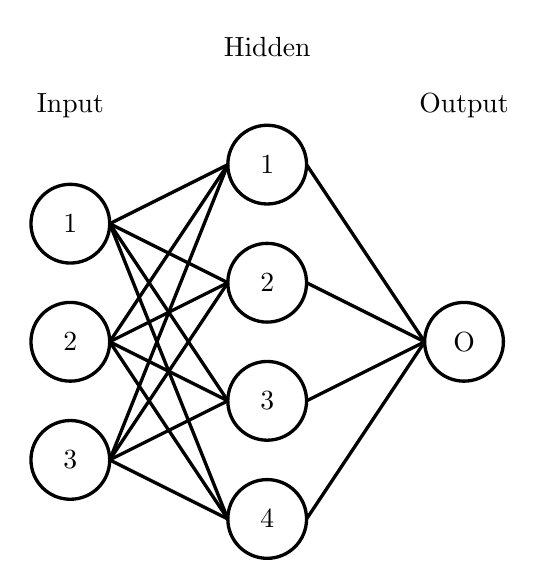
\begin{tikzpicture}

        \foreach \x in {1, 2, 3}
        {
                \draw[very thick] (0, -1.5*\x) circle (0.5);
                \node at (0, -1.5*\x) {\x};
                \foreach \y in {1, 2, 3, 4}
                {
                        \draw[very thick] (0.5, -1.5*\x) -- (2, -1.5*\y+0.75);
                }
        }

        \foreach \y in {1, 2, 3, 4}
        {
                \draw[very thick] (2.5, -1.5*\y+0.75) circle (0.5);
                \node at (2.5, -1.5*\y+0.75){\y};
                \draw[very thick] (3, -1.5*\y+0.75) -- (4.5, -3);
        }
        \draw[very thick] (5, -3) circle (0.5);
        \node at (5, -3){O};
        
        \node at (0, 0){Input};
        \node at (2.5, 0.75){Hidden};
        \node at (5, 0){Output};

\end{tikzpicture}
\end{center}
\normalsize

\end{figure}

Figur 2 er et eksempel på et meget simpelt netværk der er kendt som et Feed Forward Artificial Neural Network, eller FFANN.
Her bliver alle neuroner delt op i forskellige lag, i det her eksempel er der 3, men der kunne også være flere. Det første lag
kaldes for "Input layer", det sidste kaldes for "Output layer" og alle imellem kaldes for "Hidden layers". Så er inputtet
til hver neuron outputtet fra alle neuroner i sidste lag. Grunden til at alle neuroner i et givent lag så ikke har den samme værdi
idet deres værdi afhænger af samme neuroner, er fordi de alle sammen har forskellige vægte. Så f.eks. har første neuron 4 forskellige vægte,
én til hver af neuronerne i næste lag\footcite{ANN11}. Allerede i dette meget simple netværk er der ret rodet i forhold til de små tilslutninger mellem neuronerne.
Så derfor er det smart at have en god systematisk navngivning til de forskellige elementer der opgør et neuralt netværk.\\
Følgende navngivning vil blive brugt.\\
Neuroner(Hvor indexet 0 betyder bias:\\
Input: $I_{i}$~~~~Hidden: $H_{i}$~~~~Output: $O_{i}$ \\
Vægte har i indekset 2 numre, et nummer for hvilken neuron de er fra, og et nummer for hvilken neuron de skal til, derudover også  en indeks der viser hvilket lag de er fra
$w_{ij}^{l}$, så det kunne f.eks. være $w_{11}^I$, hvor vægten er fra input laget, og den går fra første neuron til første neuron af hidden laget(Igen er indekset 0 vægten til
biasset).
